% vim:autoindent:set textwidth=78:

\section{Print Composer}\label{label_printcomposer}

% when the revision of a section has been finalized, 
% comment out the following line:
% \updatedisclaimer

The print composer provides growing layout and printing
capabilities. It allows you to add elements such as the QGIS map canvas, 
legend, scalebar, images, and text labels. You can size, group 
and position each element and adjust the properties to create your layout. 
The result can be printed (also to Postscript and PDF), exported to image 
formats or to SVG.\footnote{Export to SVG supported, but it is not working 
properly with some recent QT4 versions. You should try and check individual 
on your system} See a list of tools in table~\ref{tab:printcomposer_tools}:

\begin{table}[h]\index{Print composer!tools}
\centering
\caption{Print Composer Tools}\label{tab:printcomposer_tools}\medskip
 \begin{tabular}{|l|p{6.9cm}|l|p{6.9cm}|}
 \hline \textbf{Icon} & \textbf{Purpose} & \textbf{Icon} &
 \textbf{Purpose} \\

 \hline 
\includegraphics[width=0.7cm]{mActionExportMapServer}
 & Export to an image format & 
 
\includegraphics[width=0.7cm]{mActionSaveAsSVG} & Export print composition 
 to SVG \\
 \hline 
\includegraphics[width=0.7cm]{mActionFilePrint} & Print or 
 export as PDF or Postscript &
 
\includegraphics[width=0.7cm]{mActionZoomFullExtent} & Zoom to
 full extend \\
 \hline 
\includegraphics[width=0.7cm]{mActionZoomIn} & Zoom in &
 
\includegraphics[width=0.7cm]{mActionZoomOut} & Zoom out \\
 \hline 
\includegraphics[width=0.7cm]{mActionDraw} & Refresh 
 view &
 
\includegraphics[width=0.7cm]{mActionAddRasterLayer} & Add 
 new map from QGIS map canvas \\
 \hline 
\includegraphics[width=0.7cm]{mActionSaveMapAsImage} & Add Image to 
 print composition &
 
\includegraphics[width=0.7cm]{mActionLabel} & Add label to print composition \\
 \hline 
\includegraphics[width=0.7cm]{mActionAddLegend} & Add new legend to 
 print composition & 
 
\includegraphics[width=0.7cm]{mActionScaleBar} & Add new scalebar to print
 composition\\
 \hline 
\includegraphics[width=0.7cm]{mActionSelectPan} & Select/Move item in 
 print composition &
 
\includegraphics[width=0.7cm]{mActionMoveItemContent} & Move content within
 an item \\
 \hline 
\includegraphics[width=0.7cm]{mActionGroupItems} & Group items of 
 print composition & 
 
\includegraphics[width=0.7cm]{mActionUngroupItems} & Ungroup items of print 
 composition \\
 \hline 
\includegraphics[width=0.7cm]{mActionRaiseItems} & Raise selected
 items in print composition &
 
\includegraphics[width=0.7cm]{mActionLowerItems} & Lower selected items 
 in print composition \\
 \hline 
\includegraphics[width=0.7cm]{mActionMoveItemsToTop} & Move selected
 items to top & 
 
\includegraphics[width=0.7cm]{mActionMoveItemsToBottom} & Move selected
 items to bottom \\
\hline
\end{tabular}
\end{table}

To access the print composer, click on the \toolbtntwo{mActionFilePrint}{Print}
button in the toolbar or choose \mainmenuopt{File} > \dropmenuopttwo{mActionFilePrint}{Print Composer}.

\subsection{Using Print Composer}\label{label_useprintcomposer} 

Before you start to work with the print composer, you need to load some 
raster and vector layers in the QGIS map canvas and adapt their properties 
to suite your own convinience. After everything is rendered and symbolized to 
your liking you click the \toolbtntwo{mActionFilePrint}{Print Composer} icon.

\begin{figure}[ht]
   \begin{center}
   \caption{Print Composer \nixcaption}\label{fig:print_composer_blank}\smallskip
   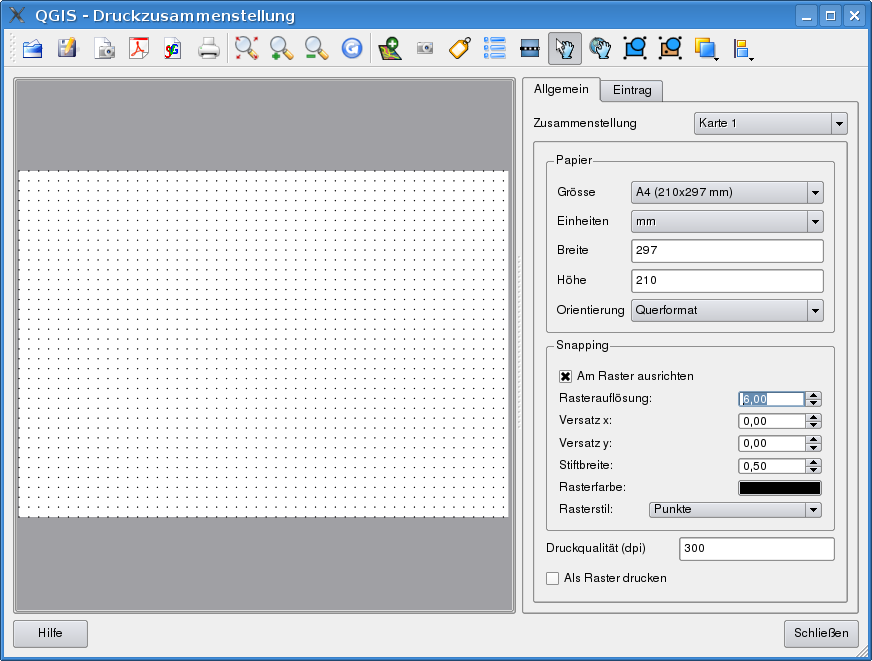
\includegraphics[clip=true, width=\textwidth]{print_composer_blank}
\end{center}  
\end{figure}

Opening the print composer provides you with a blank canvas to which you can 
add the current QGIS map canvas, legend, scalebar, images and text. Figure
\ref{fig:print_composer_blank} shows the initial view of the print composer 
before any elements are added. The print composer provides two tabs:

\begin{itemize}
\item The \tab{General} tab allows you to set paper size, orientation, and the 
print quality for the output file in dpi.
\item The \tab{Item} tab displays the properties for the selected map element. 
Click the \toolbtntwo{mActionSelectPan}{Select/Move item} 
icon to select an element (e.g. legend, scalebar or label) on the canvas. 
Then click the Item tab and customize the settings for the selected 
element.
\end{itemize}

You can add multiple elements to the composer. It is also possible to have 
more than one map view or legend or scalebar in the print composer canvas. 
Each element has its own properties and in the case of the map, its own 
extent.

\subsubsection{Adding a current QGIS map canvas to the Print Composer}

To add the QGIS map canvas, click on the \toolbtntwo{mActionAddRasterLayer}{Add new map 
from QGIS map canvas} button in the print composer toolbar and drag a 
rectangle on the composer canvas with the left mouse button to add the map. 
You will see an empty box with a \textit{"Map will be printed here"} message.
To display the current map, choose \selectstring{Preview}{Cache} in the map \tab{Item} tab.

\begin{figure}[ht]
\centering
\caption{Print Composer map item tab content \nixcaption}\label{fig:print_composer_map_item}
   \subfigure[Width, height and extend dialog] {\label{subfig:print_composer_map_item1}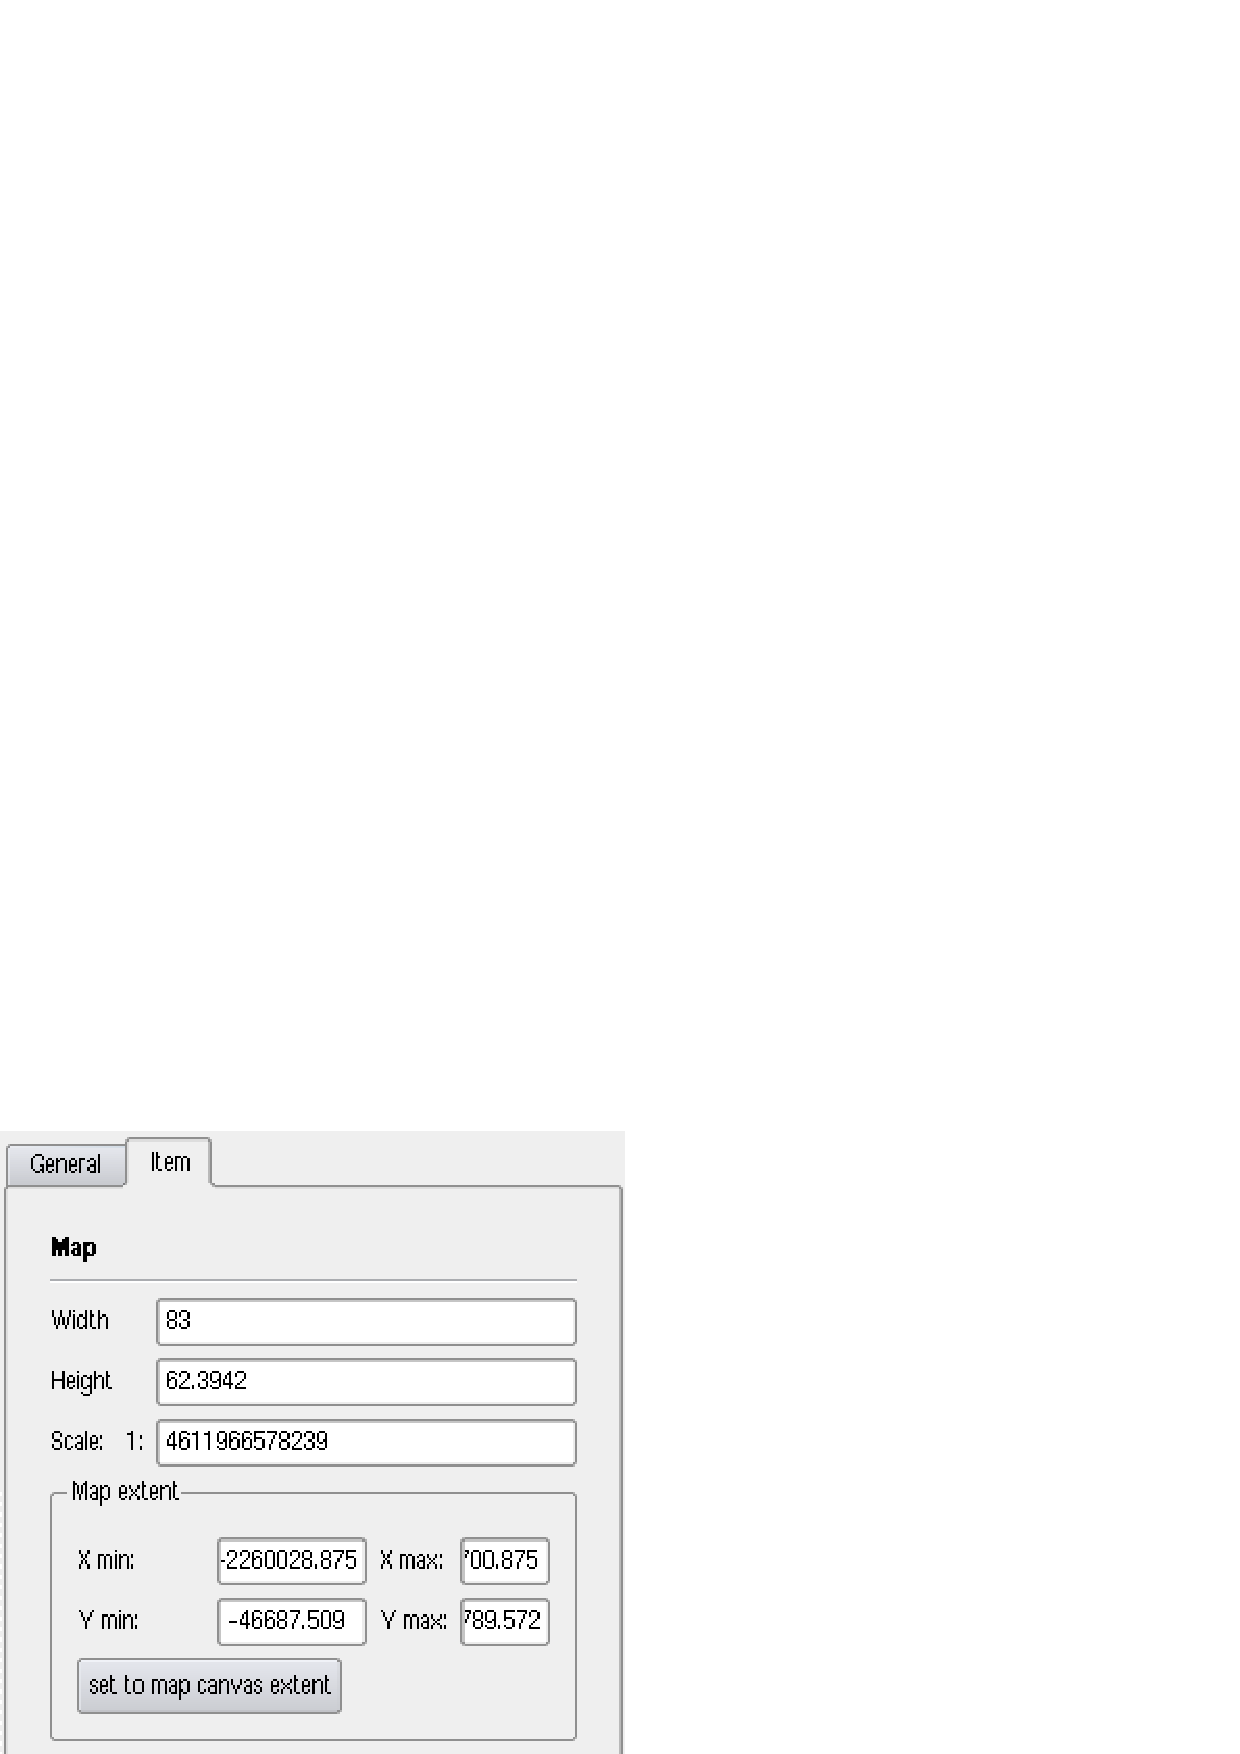
\includegraphics[clip=true, width=0.4\textwidth]{print_composer_map_item1}}\goodgap
   \subfigure[Properties dialog] {\label{subfig:print_composer_map_item2}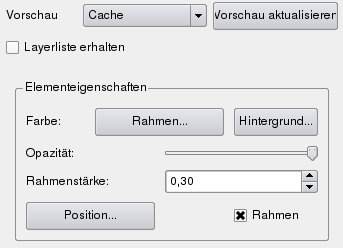
\includegraphics[clip=true, width=0.4\textwidth]{print_composer_map_item2}}
\end{figure}

You can resize the map later by clicking on the \toolbtntwo{mActionSelectPan}{Select/Move item} 
button, selecting the element, and dragging one of the blue handles in the corner of the map. With the 
map selected, you can now adapt more properties in the map \tab{Item} tab. Resize the map 
item specifying the width and height or the scale. Define the map extend using Y and 
X min/max values or clicking the \button{set to map canvas extend} button. Update the 
map preview and select, whether to see a preview from cache or an empty rectangle with 
a \textit{"Map will be printed here"} message. Define colors and outline width for the 
element frame, set a background color and opacity for the map canvas. And you can also 
select or unselect to display an element frame with the \checkbox{frame} checkbox 
(see Figure~\ref{fig:print_composer_map_item}). If you change the view on the QGIS 
map canvas by zooming or panning or changing vector or raster properties, you can 
update the print composer view selecting the map element in the print composer and clicking 
the \button{Update Preview} button in the map \tab{Item} tab 
(see Figure~\ref{fig:print_composer_map_item}). 

To move layers within the map element select the map element, click 
the \toolbtntwo{mActionMoveItemContent}{Move item content} icon 
and move the layers within the map element frame with the left mouse button.

\begin{Tip}\caption{\textsc{Saving a print composer layout}}
\qgistip{If you want to save the current state of a print composer session, click 
on \mainmenuopt{File} > \dropmenuopttwo{mActionFileSaveAs}{Save Project As} to save 
the state of your workspace including the state of the current print composer session. 
It is planned but currently not possible to save print composer templates itself.
}
\end{Tip} 

\subsubsection{Adding other elements to the Print Composer} 

Besides adding a current QGIS map canvas to the Print Composer, it is also possible 
to add, move and customize legend, scalebar, images and label elements.

\minisec{Label and images}

To add a label or an image, click the \toolbtntwo{mActionLabel}{Add label} or 
\toolbtntwo{mActionSaveMapAsImage}{Add image} icon and place the element 
with the left mouse button on the print composer canvas.

\begin{figure}[ht]
\centering
\caption{Customize print composer label and images \nixcaption}\label{fig:print_composer_tab2}
   \subfigure[label item tab] {\label{subfig:print_composer_label_item}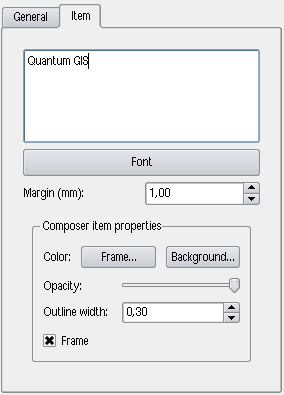
\includegraphics[clip=true, width=0.4\textwidth]{print_composer_label_item}}\goodgap
   \subfigure[image item tab] {\label{subfig:print_composer_image_item}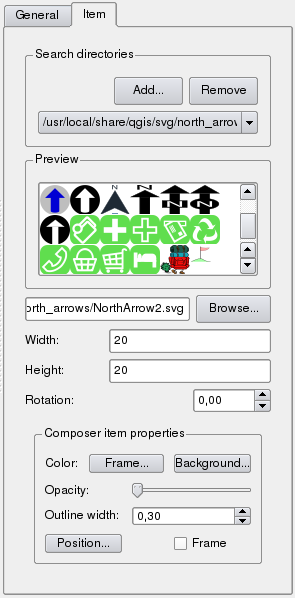
\includegraphics[clip=true, width=0.4\textwidth]{print_composer_image_item}}
\end{figure}

\minisec{Legend and scalebar}

To add a map legend or a scalebar, click the \toolbtntwo{mActionAddLegend}{Add new legend} or 
\toolbtntwo{mActionScaleBar}{Add new scalebar} icon and place the element with the left 
mouse button on the print composer canvas.

\begin{figure}[ht]
\centering
\caption{Customize print composer legend and scalebar \nixcaption}\label{fig:print_composer_tab1}
   \subfigure[legend item tab] {\label{subfig:print_composer_legend_item}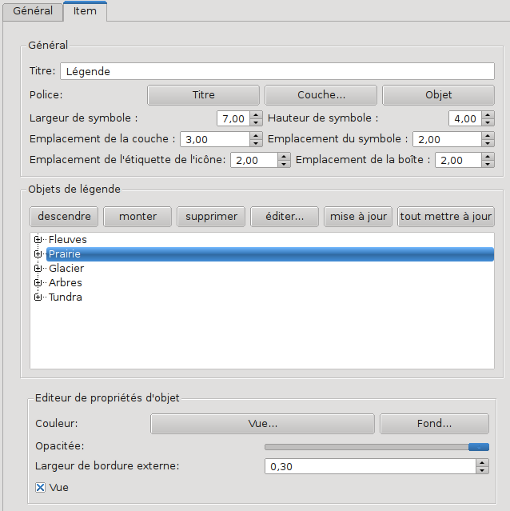
\includegraphics[clip=true, width=0.4\textwidth]{print_composer_legend_item}}\goodgap
   \subfigure[scalebar item tab] {\label{subfig:print_composer_scalebar_item}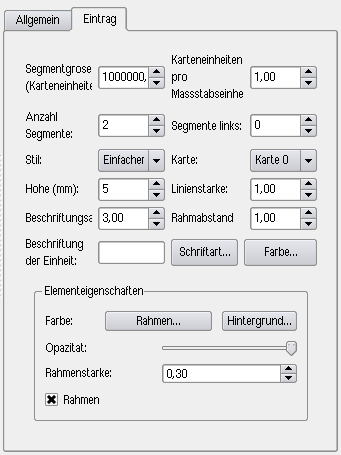
\includegraphics[clip=true, width=0.4\textwidth]{print_composer_scalebar_item}}
\end{figure}

\subsubsection{Navigation tools}

For map navigation the print composer provides 4 general tools:

\begin{itemize}
\item \toolbtntwo{mActionZoomOut}{Zoom in},
\item \toolbtntwo{mActionZoomOut}{Zoom out},
\item \toolbtntwo{mActionZoomFullExtent}{Zoom to full extend} and
\item \toolbtntwo{mActionDraw}{Refresh the view}, if you find the view in an inconsistent state. 
\end{itemize}

\subsubsection{Creating Output}

Figure \ref{fig:print_composer_complete} shows the print composer with an example 
print layout including each type of map element described in the sections above.

\begin{figure}[h]
   \begin{center}
   \caption{Print Composer with map view, legend, scalebar, and text added \nixcaption}
   \label{fig:print_composer_complete}\smallskip
   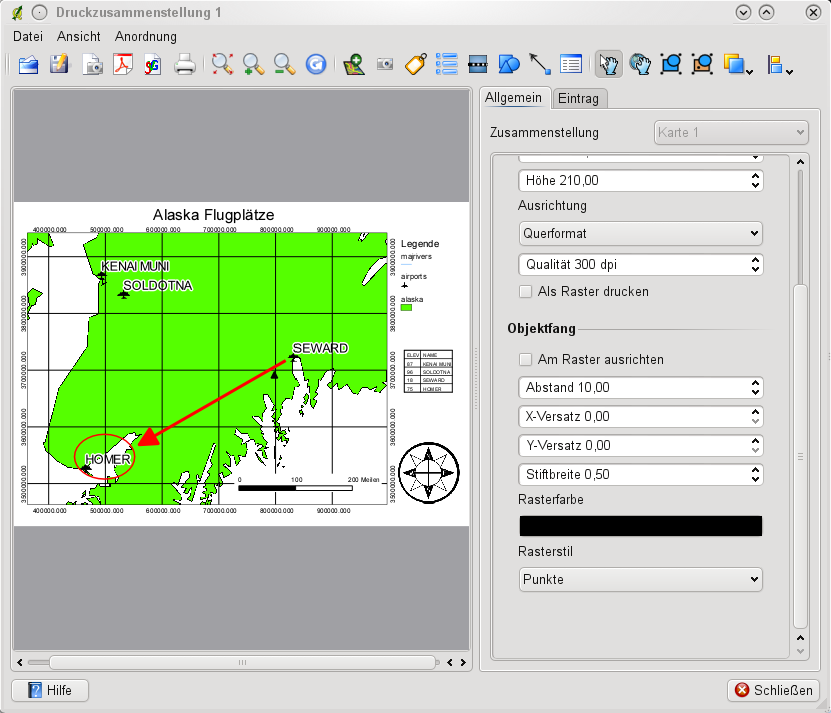
\includegraphics[clip=true, width=\textwidth]{print_composer_complete}
\end{center}  
\end{figure}

The print composer allows you to create several output formats and it is possible to 
define the resolution (print quality) and paper size:

\begin{itemize}
\item The \toolbtntwo{mActionFilePrint}{Print} icon allows to print the layout 
to a connected printer or as PDF or Postscript file depending on installed printer 
drivers.
\item The \toolbtntwo{mActionExportMapServer}{Export as image} icon exports the 
composer canvas in several image formats such as PNG, BPM, TIF, JPG, \dots
\item The \toolbtntwo{mActionSaveAsSVG}{Export as SVG} icon saves the print 
composer canvas as a SVG (Scalable Vector Graphic). \textbf{Note:} Currently the 
SVG output is very basic. This is not a QGIS problem, but a problem of the underlaying 
Qt library. This will hopefully be sorted out in future versions.
\end{itemize}

